
%----------------------------------------------------------------------------------------
%	PACKAGES AND THEMES
%----------------------------------------------------------------------------------------

\documentclass{beamer}
\mode<presentation> {
\usetheme{Berlin}
}
\AtBeginSection[]{
  \begin{frame}
  \vfill
  \centering
  \begin{beamercolorbox}[sep=8pt,center,shadow=true,rounded=true]{title}
    \usebeamerfont{title}\insertsectionhead\par%
  \end{beamercolorbox}
  \vfill
  \end{frame}
}
\usepackage{graphicx} % Allows including images
\usepackage{booktabs} % Allows the use of \toprule, \midrule and \bottomrule in tables

%----------------------------------------------------------------------------------------
%	TITLE PAGE
%----------------------------------------------------------------------------------------
\titlegraphic{
\includegraphics[width=3.5cm]{photo/logo}}

\title{IT-Projekt - Autonmously driving Remote Control Car} % The short title appears at the bottom of every slide, the full title is only on the title page
\author{Bohnstedt Timo ,
      L\"ohr Tim and Palpanes Ionannis\\%
      } 
\institute[Computer Science| Prof. Dr. Florian Gallwitz] % Your institution as it will appear on the bottom of every slide, may be shorthand to save space
{
Georg Simon Ohm University of Applied Science\\ % Your institution for the title page
\medskip
\textit{IT Project Presentation} 
}
\date{\today} % Date, can be changed to a custom date
%----------------------------------------------------------------------------------------
\begin{document}

\begin{frame}
\titlepage % Print the title page as the first slide
\end{frame}
%----------------------------------------------------------------------------------------
\begin{frame}
\frametitle{Overview} % Table of contents slide, comment this block out to remove it
\tableofcontents % Throughout your presentation, if you choose to use \section{} and \subsection{} commands, these will automatically be printed on this slide as an overview of your presentation
\end{frame}
%
%----------------------------------------------------------------------------------------
%	PRESENTATION SLIDES
%----------------------------------------------------------------------------------------

%------------------------------------------------
\section{Background}
%------------------------------------------------

\begin{frame}
\frametitle{Start of an equally simple business}
"Brian thought of a way to make a few bucks - turning
our place into \textit{designers bed and breakfast} - offering young
designers who come to town a place to cra during the 4 day
event, complete with wireless Internet, a small desk space,
sleeping mat, and breakfast each morning. Ha!
joe”
\begin{figure}
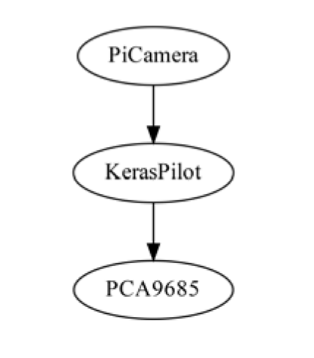
\includegraphics[width=0.4\linewidth]{photo/autonom}
\end{figure}
\end{frame}

%------------------------------------------------

\begin{frame}
\frametitle{Basics}
Airbnb is a model based on share economy. Everyone who owns an apartment can rent it out for travelers as a resting place, where it feels like home. There is a Mobile app/website: online platform to match demand and supply Listings (check in and check out: demand for short period rent apartment) .
\begin{figure}
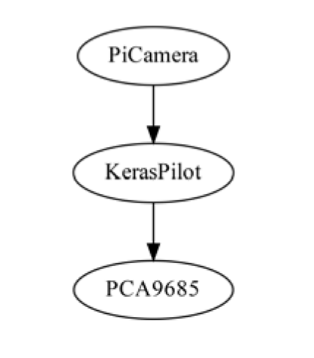
\includegraphics[width=0.4\linewidth]{photo/autonom}
\end{figure}
\end{frame}

%------------------------------------------------
\section{Literature Survey}
%---------------------------------------------
\begin{frame}
\frametitle{General Methology}
Using data analysis and show how it can be used to improve the marketing of Airbnb in Seattle according to each policy of the marketing-mix.
\end{frame}
%
%------------------------------------------------
%
\begin{frame}
\frametitle{Marketing}
\begin{columns}[c] % The "c" option specifies centered vertical alignment while the "t" option is used for top vertical alignment

\column{.45\textwidth} % Left column and width
\textbf{The 4 P's of the Marketing-Mix}
\begin{enumerate}
\item Product
\item Price
\item Promotion
\item Place
\end{enumerate}

\column{.5\textwidth} % Right column and width

\begin{block}{Definition Marketing}
Marketing is about the firm’s effort to address customer needs and expectations, which influences the demands made by the customers on the product and need to be fulfilled by the product.
\end{block}
\end{columns}
\end{frame}

%------------------------------------------------

\begin{frame}
\frametitle{How to use Data Analysis to improve the Airbnb Marketing?}
\begin{itemize}
\item \textbf{Descriptive analysis:} Reviews, locations, review and price correlation, details of listings and price correlation
\item \textbf{Descriptive analysis:} Predict the number of customer
\item \textbf{Optimization:} Optimize the booking of listings 
\item \textbf{Adaptive learning:} Learn from the results generated and combine results to give out suggestion in marketing campaigns may hold by Airbnb
\end{itemize}
\end{frame}

%------------------------------------------------
\section{Hardware}
%--------------------------------------------

\begin{frame}
\frametitle{Listings}
\begin{itemize}
\item Consist of 92 columns, with attributes describing different characteristics of the rented apartments
\item Contains 3818 apartments distributed in 79 Neighborhood
\end{itemize}
\begin{figure}
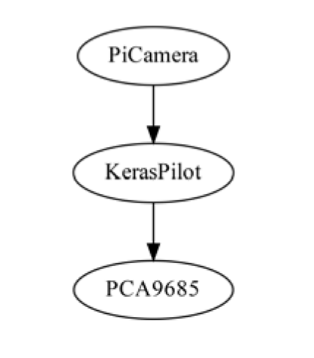
\includegraphics[width=0.8\linewidth]{photo/autonom}
\end{figure}
\end{frame}
%------------------------------------------------
\begin{frame}
\frametitle{Preprocessing Steps}
\begin{itemize}
\item Drop rows with too much sparse data (nan-values)
\item Replace nan-values with default values
\item Replace categorical with numerical features
\item Select features as input values (x) and the price as output value (y)
\item Split into training and test data (80/20)
\end{itemize}
\end{frame}

%------------------------------------------------

\begin{frame}
\frametitle{Reviews comparison}
We can see a correlation between the amount of reviews and the accommodation counts. 
\begin{figure}
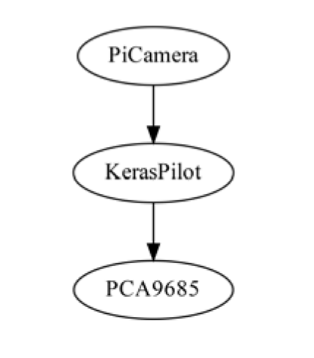
\includegraphics[width=0.8\linewidth]{photo/autonom}
\end{figure}
\end{frame}

%------------------------------------------------

\begin{frame}
\frametitle{Reviews}
\begin{itemize}
\item Apartments in total got 50 to 100 review scores and a mean rating of about 9.2 to 9.7 
\item The same mean rating is also achieved by each district where the apartments are rated between 125 and 300 times 
\item The mean rating for every district is relatively high (too positive phenomenon)
\end{itemize}
%
\begin{figure}
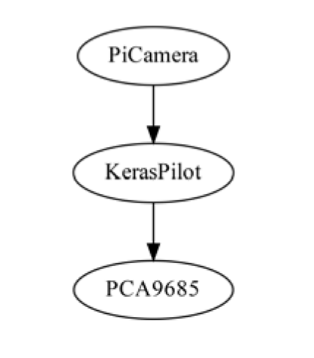
\includegraphics[width=0.8\linewidth]{photo/autonom}
\end{figure}
\end{frame}

%------------------------------------------------

\begin{frame}
\frametitle{Calendar}
\begin{itemize}
\item In January, only half of the apartments have been occupied
\item The number of rented apartments were raised until April when a sudden drop of rented apartments appeared 
\item The occupationrate raised to July and decrease again
\item The number of rented apartments have increased till December 
\end{itemize}
\begin{figure}
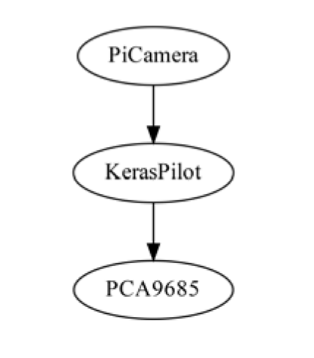
\includegraphics[width=0.8\linewidth]{photo/autonom}
\end{figure}
\end{frame}

%------------------------------------------------

\begin{frame}
\frametitle{Accumulated Listig prices}
\begin{itemize}
\item Minimum price is 10\$
\item Maximum price is 1650\$
\item Average price is 137.94\$
\item We have 669 unique values for the price among Seattle
\end{itemize}
\begin{figure}
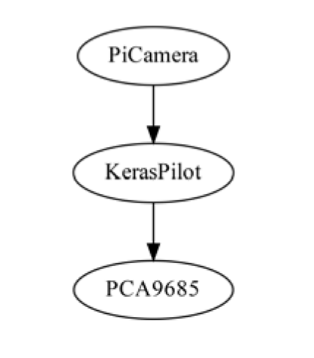
\includegraphics[width=0.8\linewidth]{photo/autonom}
\end{figure}
\end{frame}

%------------------------------------------------

%------------------------------------------------
\section{Software}
%------------------------------------------------

%------------------------------------------------

\begin{frame}
\frametitle{Natural Language Processing}
\begin{columns}[c] % The "c" option specifies centered vertical alignment while the "t" option is used for top vertical alignment

\column{.45\textwidth} % Left column and width
\begin{itemize}
\item Regular Expression Tokenizer
\item Stop Words for English + Seattle + Neighbourhood
\item Lowercase
\item WordNetLemmatizer
\end{itemize}

\column{.45\textwidth} % Right column and width
\begin{figure}
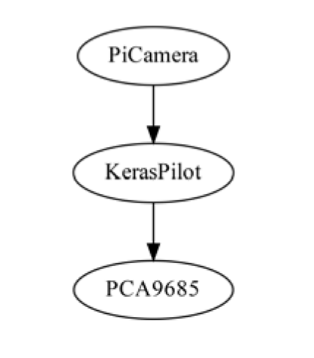
\includegraphics[width=0.8\linewidth]{photo/autonom}
\end{figure}

\end{columns}
\end{frame}

%------------------------------------------------

%------------------------------------------------

\begin{frame}
\frametitle{Linear Regression}
\begin{columns}[c] % The "c" option specifies centered vertical alignment while the "t" option is used for top vertical alignment

\column{.45\textwidth} % Left column and width
\begin{itemize}
\item Use a Linear function and estimate its parameters
\item There are different approaches to estimate the parameters
\item The accuracy of a model can be compared with different loss functions
\end{itemize}

\column{.45\textwidth} % Right column and width
The fitted line can mathematically described as:
\begin{equation}
Y_i = \beta_0 + \beta_1 X_i + \epsilon_i
\end{equation}

\end{columns}
\end{frame}

%------------------------------------------------

\begin{frame}
\frametitle{Elastic Net CV}
A general summary would be that the elastic net is a convex sum of ridge and lasso penalties, so the objective function for a Gaussian error model looks like:

\begin{block}{Mathematically defined}
\begin{equation}
\text{Residual MSE}+\alpha \cdot \text{Ridge Penalty}+(1-\alpha)\cdot \text{LASSO Penalty}
\end{equation}
\begin{equation}
1-\alpha)\cdot \text{LASSO Penalty}
\end{equation}
for \(\alpha\in[0,1]\). 
\end{block}
\end{frame}
%------------------------------------------------
\begin{frame}
\frametitle{Multinomial Naive Bayes}
\begin{columns}[c] % The "c" option specifies centered vertical alignment while the "t" option is used for top vertical alignment

\column{.45\textwidth} % Left column and width
\begin{itemize}
\item Assumes conditionally independent classes
\item Probability of observing features \(f_1\)  \\
through \(f_n\) , given some class \(c\)
\end{itemize}

\column{.45\textwidth} % Right column and width
\begin{equation}
p(f_1,..., f_n|c) = \prod_{i=1}^n p(f_i|c)
\end{equation}
This means that when I want to use a Naive Bayes model to classify a new example, the posterior probability is much simpler to work with:
\begin{equation}
p(c|f_1,...,f_n) \propto p(c)p(f_1|c)...p(f_n|c)
\end{equation}
\end{columns}
\end{frame}

%------------------------------------------------
\begin{frame}
\frametitle{LSTM Neural Network}
\begin{itemize}
\item Long Short Term Memory Neural Network is based on the Recurrent Neural Network
\item It is very well suited for timeseries analysis like the prediction of price
\item Futher explanation exceeds this presentation
\end{itemize}
\begin{figure}
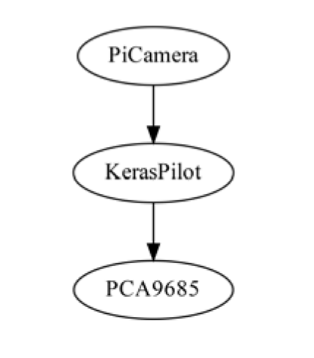
\includegraphics[width=0.8\linewidth]{photo/autonom}
\end{figure}
\end{frame}

%------------------------------------------------
\section{Machine Learning}
%--------------------------------------------
\begin{frame}
The team around Josh Keating reached a mean absolute error between 32\$ to 35\$
\begin{itemize}
\item Our network design was way to simple
\item We didn't include the important neighbourhood feature
\item Our result with our LSTM neural network was 64.04\$ (MSA)
\item Nevertheless, our best model was the linear regression with a MAE of 43.89\$
\end{itemize}
\end{frame}

%------------------------------------------------

\begin{frame}
\frametitle{Which facts lessors need to address in their description to raise the interest of potential customer, who ‘fit’ the vibe of the neighborhood and set their focus on the same aspects as former customers of these apartments?}
As shown in the word cloud:
\begin{itemize}
\item The six most reviewed cities are Capitol Hill, Ballard, Queen Anne, Belltown, Minor, Wallingford 
\item All cities have the words walk, park and restaurant written in big
\item The word “downtown” is also used often
\item For Minor, the word “lake” is very important
\item Interestingly, the word “Washington” is important for the cities Minor and Capitol Hill
\end{itemize}
\end{frame}

%------------------------------------------------

\begin{frame}
\frametitle{Which price can be charged for an apartment with certain characteristics?}
Heatmap: Correlation between features and price
\begin{figure}
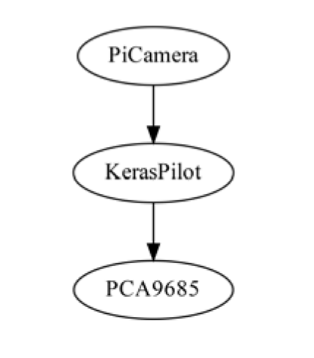
\includegraphics[width=0.8\linewidth]{photo/autonom}
\end{figure}
\end{frame}
%------------------------------------------------
\begin{frame}
\frametitle{Which price can be charged for an apartment with certain characteristics?}
As shown in the heatmap from the previous slide, there is a clear correlation between number of bedrooms and price.\\More features with correlate with the price are the beds, bathrooms, room type and guests included.
\begin{figure}
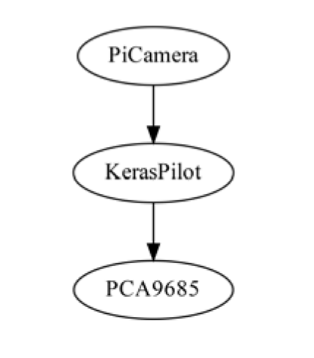
\includegraphics[width=0.8\linewidth]{photo/autonom}
\end{figure}
\end{frame}
%------------------------------------------------
\begin{frame}
\frametitle{Which price can be charged for an apartment with certain characteristics?}
Another big indicatior is the \textbf{season}. As shown in the figure below there is a strong fluctuation between the prices and the seasons.\\ So, we need to adapt our price on the current month.
\begin{figure}
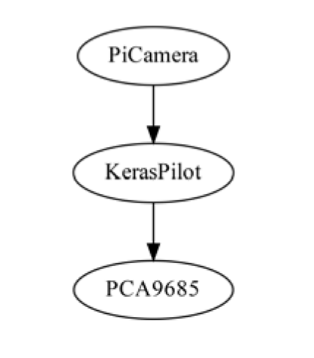
\includegraphics[width=0.8\linewidth]{photo/autonom}
\end{figure}
\end{frame}
%------------------------------------------------
\begin{frame}
\frametitle{When can lessors increase the price per night for their apartment and when should they lower it?}
\begin{itemize}
\item Price increase from January and July from 120\$ to 150\$
\item Price decrease until November to 135\$
\item We can detect an increasing demand for flats in summer time and Christmas with a correlation of an increasing price
\end{itemize}
\begin{figure}
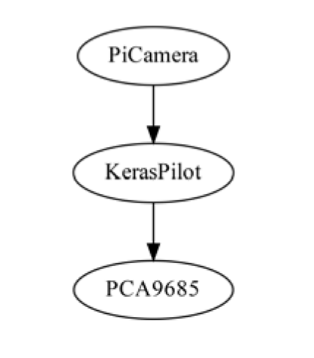
\includegraphics[width=0.8\linewidth]{photo/autonom}
\end{figure}
\end{frame}
%------------------------------------------------
\begin{frame}
\frametitle{What is a good point in time to start a marketing campaign?}
We can see clearly the high fluctuation of visitors on a weekly basis, but it is also obvious that it correlates with the picture before.\\It could be explained by people are more likely to travel on weekends than on weekdays
\begin{figure}
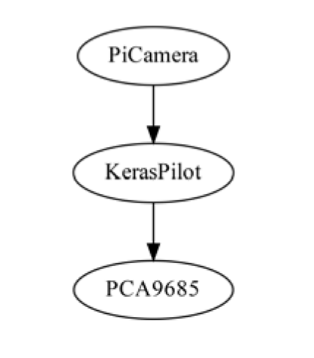
\includegraphics[width=0.8\linewidth]{photo/autonom}
\end{figure}
\end{frame}
%------------------------------------------------
\section{Deep Learning}
%------------------------------------------------
\begin{frame}
\frametitle{Our Findings and Impacts}
\begin{itemize}
\item The reviews are the most important factor of the costumers decision
\item Lessors should ask their guests to leave a review after staying at the 
\item Lessors should consider to update their description with attractive places nearby. For example a lake, park or restaurants.
\end{itemize}
\end{frame}
%------------------------------------------------
\begin{frame}
\frametitle{Our Findings and Impacts}
\begin{itemize}
\item Another big factor is how long the host has been acted and how many listings the host has
\item Hosts should try to increase their response time
\item Obviously providing more bathrooms or bedrooms leads to rent the flat for a higher price
\end{itemize}
\end{frame}
%------------------------------------------------
\section{Autonomously Driving}
%------------------------------------------------
\begin{frame}
\frametitle{Conclusion}
\begin{itemize}
\item We made some suggestions how to apply marketing-mix strategies effectively. The focus was on the Product, Price and Promotion policy which is known from the marketing definition
\item Lessors could experiment with new trendy words in their description
\item The number of bedrooms has to be exceeded to five before the entry price increased

\end{itemize}
\end{frame}
%---------------------------------------------
\begin{frame}
\frametitle{Conclusion}
\begin{itemize}
\item From January until July lessor should increase their price but decrease again until November
\item On Christmas they can Increase their price
\item It make sense to start the marketing campaign in February to be noticed before the rising customer counts
\end{itemize}
\end{frame}
%---------------------------------------------
\begin{frame}
\frametitle{References}
For references pleace look in the origin report "How can the effectivness of marketing 'Airbnb Seattle' be improved? - dataset of 2016 
\end{frame}
%------------------------------------------------
\begin{frame}
\Huge{\centerline{-- The End -- }} 
\vspace{5mm}
\begin{center}
	
\includegraphics[width=4cm]{photo/logo}
\end{center}
\end{frame}
%----------------------------------------------------------------------------------------

\section{Evaluation}
%------------------------------------------------
\begin{frame}
\frametitle{Conclusion}
\begin{itemize}
\item We made some suggestions how to apply marketing-mix strategies effectively. The focus was on the Product, Price and Promotion policy which is known from the marketing definition
\item Lessors could experiment with new trendy words in their description
\item The number of bedrooms has to be exceeded to five before the entry price increased

\end{itemize}
\end{frame}
%---------------------------------------------
\begin{frame}
\frametitle{Conclusion}
\begin{itemize}
\item From January until July lessor should increase their price but decrease again until November
\item On Christmas they can Increase their price
\item It make sense to start the marketing campaign in February to be noticed before the rising customer counts
\end{itemize}
\end{frame}
%---------------------------------------------
\begin{frame}
\frametitle{References}
For references pleace look in the origin report "How can the effectivness of marketing 'Airbnb Seattle' be improved? - dataset of 2016 
\end{frame}
%------------------------------------------------
\begin{frame}
\Huge{\centerline{-- The End -- }} 
\vspace{5mm}
\begin{center}
	
\includegraphics[width=4cm]{photo/logo}
\end{center}
\end{frame}
%----------------------------------------------------------------------------------------

\end{document} 